\chapter{An Introduction to Knotted Fields}

\section{Kelvin's vortex atom}
\label{sec:Kelvin}
The original, and perhaps most familiar, example of a knotted field is the smoke ring. Easily made by cutting a circular hole in a rectangular box, then replacing the opposite side entirely with a sheet of rubber, ``a blow on this flexible side causes a circular vortex ring to shoot out from the hole on the other side'' \citep{Kelvin}. In 1867, exactly this demonstration was shown to Lord Kelvin by Peter Guthrie Tait. What is generated is a tightly circulating tube of air, closed into a ring, which propagates stably across the room, rebounding elastically from walls and even other vortex rings (of course to see the ring one first needs to fill the box with smoke, perhaps using dry ice or ``a small quantity of muriatic acid'' \citep{Kelvin}). At the time, the microscopic nature of atoms was still under debate, and the stability of the rings, a consquence of Helmholtz's laws of vortex motion in an ideal fluid \citep{Helmholtz} (translated into English by Tait), coupled with their elasticity and capacity for internal vibration \citep{KelvinMasters, KelvinAMS} prompted Kelvin to suggest that ``Helmholtz's rings are the only true atoms". Kelvin hypothesised that such rings, embedded in a ``perfect homogenous liquid''\footnote{Kelvin did not actually specify whether this fluid was the same as the `ether' hypothesised to transmit electromagnetic waves \citep{KelvinMasters}.}, and ``linked together or ...knotted in any manner'' might form the microscopic basis of all matter \citep{Kelvin}.
\begin{figure}[htbp]
\centering
\includegraphics[width=0.99\linewidth]{\IntroductionFigures/History.pdf}
\caption{hi }
\label{fig:History}
\end{figure}

Kelvin's ``vortex atom'' rapidly encountered difficulties in its mathematical content, its falsifiability, and a lack of contempory experimental support \citep{KelvinMasters}. However its content, summarised as ``\textit{Physics = Geometry}'' in Ref. \citep{KelvinAMS}, was compelling (perhaps slightly dangerously so) and apparently motivated Tait, in ``consideration of the forms of knots by Sir W. Thomson's (Lord Kelvin) Theory of Vortex Atoms'', to construct the first systematic tables of knots in 1876--1885 (Figure \ref{fig:History}) \citep{Tait1, Tait2, Tait3}. Tait's articles, alongside a ``very remarkable essay by Listing ... and an acute remark made by Gauss ... with some comments on it by Clerk-Maxwell'' \citep{Tait}form the initial studies in  what is now the mathematical field of Knot Theory \cite{Lickorish}. Maxwell himself, although not an active contributor to vortex atom theory, had a clear interest in the ideas, encouraging Tait and Kelvin to ``prosper and disentangle your formulae in proportion as you entangle your worbles'' (Figure \ref{fig:History}) \citep{MaxwellTaitLetter}. Indeed the ``comments by Clerk-Maxwell'' referred to by Tait are in fact Maxwell's rederivation of Gauss's Linking number, as presented in his \textit{A Treatise on Electricity and Magnetsim} in 1873, about which we will have much more to say in \ref{ch2}. 

Despite forming the starting point for modern knot theory, the knotted structures above are quite different to those found in your shoelaces, or in the world of art and design outside the physics department\footnote{or so I am told.}. Rather than a single knotted curve, we have a continuous fluid in whose structure the knot is encoded, and from which dynamical properties of the knot (its motion, stability, a spectrum of vibrational modes etc.) may be derived. More precisely, we have a concentrated tube of vorticity in the fluid, tied into the shape of a knot. Helmholtz's laws of vortex motion demonstrated that, in a perfect (frictionless) fluid this tube of vorticity was `frozen in' to the fluid, unable to dissapate or cross itself. In an idealised vortex atom, the radius of this tube would tend to zero, with the vorticity contained inside becoming infinite, and we would have a singular linelike structure, tied into a knot and embedded into a continuous three dimensional medium. This structure is our first example of what is called a \emph{knotted field}. There is no strict definition of what constitutes of a knotted field, but a sensible effective one is that they are physical fields containing knotted, linked, or otherwise topologically interesting structure, and that this structure has some interplay with the behaviour of the whole field. As we shall see, such fields are not certainly not confined to fluids.

The disconnect between a knotted curve and a knotted field is reflected in Tait's work, which mentions Kelvin's Vortex Atoms briefly as motivation, but focuses in substance on ``\emph{the investigation of the essentially different modes of joining points in a plane}'' \citep{Tait1}. As knot theory developed, its initial connections to hydrodynamics and electromagnetism were further abandoned. We also note that despite the wonderful knot tables produced by Tait (figure \ref{fig:History}) and the reliance of vortex atom theory on knotted and linked vortices, there is no mention above of any experimental evidence of vortices tied in nontrivial knots. 
\begin{figure}[htbp]
\centering
\includegraphics[width=1 \linewidth]{\IntroductionFigures/Irvine_Figs1_3.pdf}
\caption{hi }
\label{fig:Irvine}
\end{figure}

The first experimental construction of nontrivial knotted fluid vortices came 140 years after their initial theoretical investigation, from the Irvine lab in 2013 --- we show in figure \ref{fig:Irvine} several remarkable figures reproduced from Ref.~\citep{Kleckner2013}, in which Kleckner et al. tied a single vortex in water into a trefoil knot, the simplest nontrivial knot, as well as linking two vortex loops together (Kelvin's proposed model for a Sodium atom), before tracking their evolution in full 3D. Ref.~\citep{Kleckner2013} is a noteable example of a more general trend; over the past $\sim10$ years knotted fields have gone from being purely theoretical constructions to being experimentally realisable in a number of systems, and though originally concieved of in fluid dynamics, modern applications are not limited to this context; they have been realised as nodal lines of optical beams~\citep{Dennis2010}, as disclinations in nematic liquid crystals and as spinor Bose-Einstein condensates~\citep{Tkalec2011,Tasinkevych2014,Copar2015}. In the next section we will review the state of modern experiment and theory on knotted fields, beginning with fluids and superfluids --- in some sense the most developed case --- before moving on to parallel developments in liquid crystals and excitable media, which directly underlie the work in \S\S \ref{ch:FitzHughNagumo} and \S\S \ref{ch:TwistBendNematic} in this Thesis. We shall see that the subject has broadened considerably since Kelvin's atoms and the study of fluids. There will be a commonality of ideas between the different disciplines mentioned above, but also geniuine differences.

\section{Modern knotted fields: Fluids}
\label{sec:Fluids}
With the decline of Kelvin's vortex atom theory and the development of knot theory away from its hydrodynamic origins, a resurgence of interest in knotted fields might be dated to the years 1958-1969, with Moreau and Moffatt's seminal papers on Helicity in ideal fluids \cite{Moreau,Moffat}, preceded by analogous results in magnetohydrodynamics by Woltjer \cite{Woltjer}. Focusing on the ideal fluid, both Moreau and Moffatt independently demonstrated that the Helicity

\begin{equation}
    \mathcal{H} = \int {\bf u} \cdot {\boldsymbol{\omega}} \ d^3 \bf r,
\end{equation}
where ${\bf u}({\bf r},t)$ is the fluid velocity and $\boldsymbol{\omega} = \nabla \times \bf u$ is the vorticity \cite{Saffman}, is conserved under the Euler equations of ideal flow. Moffatt in particular gave this invariant a topological interpretation: it measures the linking of vortex tubes within the fluid. Given a fluid where $\omega$ is concentrated along discrete sets of curves $C_i$, Moffat showed that
\begin{equation}
    \mathcal{H} = \sum_{i,j, i\neq j} Lk(C_i,C_j) \Gamma_i \Gamma_j 
\end{equation}
where $\Gamma_i$ is the vorticity flux of along curve $C_i$, and $Lk(C_i,C_j)$ is the Gauss Linking number between curves $C_i, C_j$ (this interpretation of Helicity actually extends to the case where the vorticity is not concentrated along a finite set of curves, but is distributed throughout the fluid \cite{Arnold,Berger,Berger}). Figure \ref{fig:Moffat} shows several examples of vortex tubes with different linking numbers and hence helicities. Seen in this light, the conservation of Helicity is a direct consequence of Helmholtz's laws of vortex motion, and is equivalent to the statement that initially linked vortex tubes remain so; in some sense it is remarkable that the result was not known to Kelvin and Maxwell.
\begin{figure}[htbp]
\centering
\includegraphics[width=1 \linewidth]{\IntroductionFigures/Moffat.pdf}
\caption{hi }
\label{fig:Moffat}
\end{figure}

When vorticity is not concentrated along a singular curve but distributed in a thin vortex tube, there is additional internal structure --- one imagines a knotted ribbon (Figure \ref{fig:RibbonMontage}(a)), or rubber bicycle tyre (Figure \ref{fig:RibbonMontage}(b)). Flux lines may wind around the centre-line of this tube as in Figure \ref{fig:RibbonMontage}(b), endowing it with a second linking number, the Self-Linking number, which measures the linking of any flux line with the curve centre-line, or equivalently the number of rotations any flux line makes as we traverse the centre-line once. 
\begin{figure}[htbp]
\centering
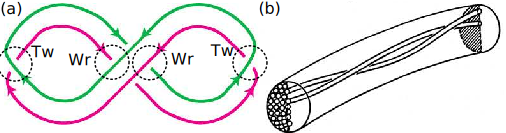
\includegraphics[width=\linewidth]{\IntroductionFigures/RibbonMontage.pdf}
\caption{hi }
\label{fig:RibbonMontage}
\end{figure}
Incorporating this structure into the helicity count we find \cite{MoffatRicca}
\begin{equation}
    \mathcal{H} = \sum_{i,j, i\neq j} Lk(C_i,C_j) \Gamma_i \Gamma_j + \sum_{i} \Gamma_i^2 SL(C_i) 
    \label{eq:HelicityCount}
\end{equation}
where $SL(C_i)$ denotes the self linking of each curve $C_i$ with its implicitly assumed ribbon. 

\subsection{Calugareanu's Theorem, Real fluids}
Given a ribbon diagram like figure \ref{fig:RibbonMontage}(a), the self linking number of may be further decomposed as
\begin{equation}
    SL = Tw + Wr.
    \label{eq:Count}
\end{equation}
The first term, the twist $Tw$, counts the local crossings of the ribbon over its centre-line. The second term, the writhe $Wr$, counts non-local crossings of the ribbon over distant parts of the centre line. In figure \ref{fig:RibbonMontage} each crossing of the ribbon over its centre-line is annotated with the nature of its contribution. Note that the $Wr$ count is actually independent of the choice of ribbon. For different diagrams of the same knotted ribbon each of these contributions varies, but their sum $SL$ does not. Averaging over also possible diagrams, i.e. all possible projections of the geniuine three-dimensional curve, one obtains integral formulae for twist and writhe, and in this form the result eq. \ref{eq:Count} was first discovered by Georges Calugareanu \cite{Cal} (the interpretation of it given above is however due to Ref.~\cite{Dennis}). Calagareanu's Theorem is an important and influential result, finding application in Mathematics, Physics, Biology and beyond. It is of potential relevance whenever one studies the properties of a curve with some internal structure, and so it naturally appears frequently in the study of knotted fields. It will play a role in the curve dynamics studied in \S\S\ref{ch3} and, in its close connection to Maxwell and Gauss's work on linking numbers and electromagnetism, in \S\S\ref{ch2} as well. For the purposes of the current discussion it enables us to speak of \emph{writhe} helicity and \emph{twist} helicity, two seperate contributions to the total helicity count.    

In a real (viscous) fluid, helicity is not \emph{a priori} conserved. The question of whether it is in practice, and the mechanism of its dissipation, are areas of active research and motivation for the experiments shown in Figure \ref{fig:Irvine} \cite{Klecker}. The reconnections shown in figure \ref{fig:Irvine} suggest that helicity is not conserved, however experiments tracking its evolution in detail \cite{Kleckner,Kleckner,Scheeler} find that this is not the case. Instead, reconnections transfer the initial linking of curves (c.f. eq. \ref{eq:HelicityCount}) into self linking, preserving total helicity to a remarkable extent. More precisely, what is conserved is the sum $Lk +Wr$, with the helicity in $Lk$ being transferred to $Wr$ at a reconnection; the twist helicity $Tw$ is dissipated by viscosity (figure \ref{fig:Irvine2}).
\begin{figure}[htbp]
\centering
\includegraphics[width=0.7\linewidth]{\IntroductionFigures/Irvine2.pdf}
\caption{hi }
\label{fig:Irvine2}
\end{figure}

\subsection{Fluids as a case study}
The hydrodynamic (and magnetohydrodynamic) story of knotted fields is well developed. We have given a sketch, but the reader is invited to find more detail in reviews such as Refs. \cite{Moffat, Irvine}. Outside of hydrodynamics the above discussion acts as a template for what one might expect in knotted fields more generally; a test case which other systems may be compared to and contrasted against. In particular, linking and self-linking of structure occur in a variety of contexts, and in an analogy to (\ref{eq:HelicityCount}) one might seek to connect them to conserved quantites, and use them to understand the dynamics of the entire system under study. To give a brief example of system for which this template is fruitful consider superfluids, close cousins of normal fluids described by a complex scalar field $\psi = |\psi| e^{i \phi}$ (Figure \ref{fig:SuperFluidMontage}(a)) evolving via the non-linear Schroedinger equation \cite{scheeler}. Here vortices are given by singular lines where the circle-valued phase field $\phi$ is undefined, and about which it winds by $2\pi$. As in fluids, one may define some notion of helicity (although its precise form is more ambiguous than is the case in fluids \cite{Salman}), initialise knotted vortices and study their evolution (figure \ref{fig:SuperFluidMontage}(b)) \cite{Scheeler}. The helicity evolution turns out to be remarkably similar to that of real fluids \cite{Scheeler}; reconnections occur in a manner similar to thse found in real fluids, and they preserve the combination $Lk+Wr$.  
\begin{figure}[htbp]
\centering
\includegraphics[width=\linewidth]{\IntroductionFigures/SuperFluidsMontage.pdf}
\caption{hi }
\label{fig:SuperFluidMontage}
\end{figure}

However, it is not the case that knotted fields in other systems may be understood simply through the lens of fluids. In the following section we turn to the second experimental system with which substantial work on knotted fields has been done, the nematic liquid crystal cells of Refs.~\citep{Tkalec2011,Tasinkevych2014,Copar2015}. There will be some crossover with the discussion above, but also geniuine differences, especially in the theoretical constructions involved, which are of a quite different charecter. 
\section{Modern knotted fields: Liquid Crystals}
\begin{figure}[htbp]
\centering
\includegraphics[width=0.8 \linewidth]{\IntroductionFigures/LiquidCrystalMontage.pdf}
\caption{hi }
\label{fig:KnottedLiquidCrystal}
\end{figure}
A second experimentally constructed knotted field is shown in figure \ref{fig:KnottedLiquidCrystal}. It is quite different to that of figure \ref{fig:Irvine}. By including microscopic colloids a few $\mu$m wide into a thin cell of nematic liquid crystal, experimentalists~\citep{Tkalec2011,Tasinkevych2014,Copar2015} are able to force the appearance of defect lines in the material. These defects may then be manipulated with lazer tweezers, and by weaving them about an array of colloids, a knotted field encoding any type of knot or link can be constructed; unlike the fluid vortices above, these structures are stable, able to be experimentally probed in some detail. This system provides a testbed for series of new ideas about knotted fields described below, but first we step back a moment and provide a brief description of what liquid crystals, defects and colloids etc. actually are.

\subsection{A brief introduction to liquid crystals}

Liquid crystals are a class of materials which possess properties associated to both liquids and solids~\cite{DeGennes}. In their most common form, the nematic phase, they show no positional order, and flow like a liquid . However, they do show orientational order: if one attempts to twist a portion of the liquid crystal it will respond elastically, as a solid would\footnote{This is remarkable: imagine your surprise if, upon attempting to stir your coffee, you found it fiercly resisted your attempts to turn the spoon, but was nevertheless happy to be poured down the sink.}. The microscopic basis for this behaviour comes from the type of molecules which comprise nematics, two examples of which are shown in Figure \ref{fig:DeGennesMontage}; they are typically thin rods which locally align themselves along some common axis without taking on any sort of crystalline postitional order. In continuum theories this orientational order is described by a spatially varying unit vector field $\bf n$, called the director, which represents an average local molecular orientation, as shown in Figure \ref{fig:DeGennesMontage} (c).
\begin{figure}[htbp]
\centering
\includegraphics[width=1\linewidth]{\IntroductionFigures/DeGennesMontage.pdf}
\caption{hi }
\label{fig:DeGennesMontage}
\end{figure}

The theory of their elastic distortions contains much interesting geometry which we will return to in \S \ref{sec:Geometry}, but for an understanding of figure \ref{fig:KnottedLiquidCrystal} we instead focus on a celebrated feature of nematics \cite{Frank}, their topological defects. If one shines polarised light through a thin slice of nematic placed between crossed polarisers, they will observe something like figure \ref{fig:Disclination}(a), a Schlieren texture \cite{DeGennes}. Places in the sample where the director $\bf n$ is aligned with one of the two polariser directions H and V do not transmit light, leading to the dark brushes observed. One immeadiately notes points where the brushes meet, sometimes with two brushes leading into a point, sometimes four. What is the structure of the director at these points? The confluence of dark brushes implies that, in a small circle around these points, the director winds, and that at the point itself we cannot consistently define a director $\bf n$; these points are topological defects, places where the order breaks down. Traversing such a circle around a point with two brushes, the director is aligned with each of H and V only once; in other word it makes only half a turn in a full circle around the defect. This observation is enough to establish that the director $\bf{n}$ must in fact be non-orientable; it should not be thought of as a vector field, but as a line field, for which $\bf n \sim - \bf n$.
\begin{figure}[htbp]
\centering
\includegraphics[width=1\linewidth]{\IntroductionFigures/DisclinationLine.pdf}
\caption{hi }
\label{fig:Disclination}
\end{figure}
In figure \ref{fig:Disclination} (b)--(e) we show configurations of the director around these defects, with their associated Schlieren texture brushes. In (b) and (e) we have four brushes, and a line field which can be oriented; to emphasise this fact we have decorated the line field with one of the two possible choices of arrowheads. Figures (c) and (d) correspond to the non-orientable two brush case; here one cannot consistently assign arrowheads to the rods (it is worth trying to imagine doing so). Note that from a single image such as figure \ref{fig:Disclination}(a), we cannot distinguish defects winding in a right handed sense (plus in the figure) from left handed by counting brushes.  In two dimensions these defects, also called disclinations or dis\emph{in}clinations \cite{Frank}, are points, but in three dimensions they are lines, transverse cross sections of which have local profiles resembling the two dimensional case; a schematic illustration is shown in Figure \ref{fig:Disclination}(f). As with fluid vortices, these disclination lines may be knotted and linked together, and the rotation of the local profile along the disclination (see the cross sections in Figure \ref{fig:Disclination}(f)) provides internal structure giving rise to self linking.

\subsubsection{Experiments on knotted disclination lines}

We now return to the experiments of Refs~\citep{Tkalec2011,Tasinkevych2014,Copar2015}. In contrast to situation in fluids, one of the major advantages of working with liquid crystal disclinations is the control experimentalists have over them. By including microscopic silica spherical colloids (4.72 $\mu$m diamter in figure \ref{fig:KnottedLiquidCrystal}) into a sample of liquid crystal with specific surface anchoring conditions, experimentalists may frustrate alignment of the director $\bf n$ in a controlled fashion, neccesitating the appearance of disclination lines \cite{}. For example, in a thin cell of liquid crystal treated to promote uniform alignment of $\bf n$ within the sample, the inclusion of a colloid with normal anchoring conditions forces the appearance of a defect line around it to cancel the colloid's topological charge (it effectively acts as a point defect) and $\bf n$ to relax to uniform at large distances. Two such ``Saturn's ring'' configurations may be seen in the first frame of figure \ref{fig:KnottedLiquidCrystal}(a). Once generated, these disclinations, as well as the colloids they wrap around, may be further manipulated using lazer tweezers \citep{Tkalec2011}, as shown in the remainder of figure \ref{fig:KnottedLiquidCrystal}(a). When two of these colloids are brought together the disclinations, either spontaneously or induced by the tweezers, fuse together (Figure \ref{fig:KnottedLiquidCrystal}(a), top row). Assembling an array of these colloids and weaving the disclination lines around them, the setup of Refs.~\citep{Tkalec2011,Tasinkevych2014,Copar2015} allows targeted construction of any knot or link; examples of some possible link topologies are shown in Figure \ref{fig:KnottedLiquidCrystal} (b). This system also strikingly illustrates that knotted fields have more structure than a single knotted curve; the curve organises the entire field (in this case the director $\bf n$) around it. Figure \ref{fig:KnottedLiquidCrystal}(c) shows the knotted liquid crystal coloured by whether the director is twisting in a right or left handed sense. We see that the disclinations separate the liquid crystal into alternately right and left handed regions. This division corresponds to a surface spanning the disclinations called the Pontryagin-Thom (PT) surface \cite{Chen}, shown as the coloured surfaces in figure \ref{fig:KnottedLiquidCrystal}(c), which classifies the topology of this liquid crystal texture; we shall return to it in a moment.

Let us compare the phenomena seen here to \S\ref{sec:Fluids}. Firstly, in contrast to fluid vortices, it is experimentally possible to stabilise disclinations, leading to a greater experimental and theoretical focus on their static properties than their dynamics. If not stabilised by colloids, liquid crystal disclinations shrink under effective line tension and undergo reconnections, however there is relatively little theoretical work on possible conservation laws, analogous to eq. \ref{eq:HelicityCount}, although some results do exist \cite{Machon}. In this sense the dynamics of these knotted fields is less understood than is the case in fluids. However, as well as the experimental possiblities, the focus on static knotted fields in liquid crystals is motivated by as follows: in a two dimensional fluid there is only one type of vortex, topologically speaking. In a slice of liquid crystal, however, we saw there were many types, indexed by the winding of the director. What of liquid crystal textures in three dimensions?

\subsection{The homotopy theory of knotted disclinations}
With these experimental advances comes the need for new theory. In particular, as mentioned above, for any given knotted disclination line there may in fact correspond multiple nematic textures which cannot be continuously deformed into one another, and it is desirable to have methods which classify them. The traditional method is to place a measuring surface around a defect and study the possible textures on this surface, i.e. the different classes of map from the measuring surface to the space of possible values the order takes. Maps are equivalent when a continuous deformation, also called a homotopy, exists between them, and as such this framework is known as the homotopy theory of defects \cite{Mermin,Alexander}. In a three-dimensional sample of nematic the director $\bf n$ takes values in $S^2/\{x\sim-x\}$, the sphere with antipodal points identified, also called the real projective plane $\mathbb{R}P^2$. Encircling a disclination line with a measuring loop as shown in Figure \ref{fig:RP2} the different classes are reduced to the classification of maps ${\bf n}:S^1 \rightarrow \mathbb{R}P^2$. Actually computing these classes is the work of Algebraic Topology, in which maps of a sphere $S^n$ into a space $X$ are termed the homotopy groups $\pi_n(X)$. It is found that $\pi_1(\mathbb{R}P^2) \approx \mathbb{Z}_2$ and thus there are precisely two distinct types of disclination line as far as the traditional form of the theory is concerned \footnote{Given figures \ref{fig:Disclination}(a)-(d) this result appears surprising. If the director is confined to a plane, its space of possible directions is $S^1/\{x\sim-x\} \approx \mathbb{R}P^1$.$\pi_1(\mathbb{R}P^1) \approx \mathbb{Z}$ and there are infinitely many distinct textures. However if we allow the director out of the plane of the paper, it may buckle (upwards say) in figures (a) and (d), reducing these textures to the trivial one. This ``escape in the third dimension'' causes $\mathbb{Z}$ to undergo a mod 2 reduction \cite{Machon}. }.
\begin{figure}[htbp]
\centering
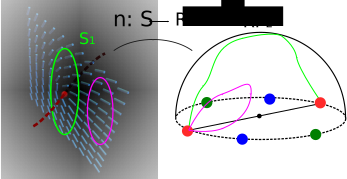
\includegraphics[width=0.9\linewidth]{\IntroductionFigures/RP2.png}
\caption{hi }
\label{fig:RP2}
\end{figure}
A limitation of this approach is that, in only considering the texture on a specific measuring surface (in practice a sphere of some dimension) it discards information about the rest of the texture, which leads to ambiguities when considering multiple defects or more complex structures such as knotted and linked disclinations \cite{Alexander,Machon}. A more recent, global approach \cite{Machon} does not fix a measuring surface, but instead classifies maps into $\mathbb{R}P^2$ where the domain the is entire liquid crystal sample $M$ minus some set of (possibly knotted and linked) disclination lines $L$. The result is that the homotopy classes of the director are given by
\begin{equation}
[M-L, \mathbb{R}P^2] \approx H_1(\Sigma(L); \mathbb{Z})/\{ x \sim -x\}
\end{equation}
where $\Sigma(L)$ is the branched double cover of the link complement (its appearance in the result is a consequence of director non-orientability), and $H_1(\Sigma(L); \mathbb{Z})$ is its first homology group. Without going into the details of this result, it is clear that these homotopy classes are far richer than the traditional classification scheme for disclinations would suggest, and that they depend strongly on the knot or link under consideration. To illustrate this point, in figure \ref{fig:MachonMontage} we reproduce a `periodic table' of possible textures for $(p,q$) torus links from Ref.~\cite{Machon}. As an example, we see that for the Hopf Link, the simplest possible link consisting of two curves passing through each other once and given by $(p,q)=(2,2)$ in figure \ref{fig:MachonMontage}, there are exactly two nonhomotopic textures. 
\begin{figure}[htbp]
\centering
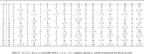
\includegraphics[width=\linewidth]{\IntroductionFigures/MachonMontage.pdf}
\caption{hi }
\label{fig:MachonMontage}
\end{figure}
\subsection{The Pontryagin-Thom Construction}
\begin{figure}[htbp]
\centering
\includegraphics[width=0.8\linewidth]{\IntroductionFigures/PontryaginThom.pdf}
\caption{hi }
\label{fig:PT}
\end{figure}
Given there exist two inequivalent hopf link textures, a natural question to ask is how one should visualise them. One solution is a construction which generalises the dark brushes of Schlieren textures to three dimensions --- the Pontryagin-Thom construction \cite{ChenThesis, GarethBook,Machon, HopfFibrationExper}, already encountered as the coloured surface bounded by disclinations shown in fig.~\ref{fig:KnottedLiquidCrystal}(c). The idea is to extract the set of all points in the sample where the director is horizontal (more generally, perpendicular to some fixed direction in $\mathbb{R}P^2$).  This is exactly what a Schlieren textures shows, although Schlieren textures contain some redundancy, showing us the set where the director is both horizontal and vertical ---  we only really need half this data. In a three dimensional sample this `horizontal set' is not comprised of lines as in the two-dimensional Schlieren texture but is a surface, the Pontryagin-Thom (PT) surface. After finding this surface, the construction is completed by coluring it according to the orientation in the horizontal plane that the director takes. An illustration of this procedure is shown in figure \ref{fig:PT}(a). A powerful result in Algebraic Topology called the Pontryagin-Thom correspondance \cite{Milnor, Hatcher} shows that these coloured surfaces, taken up to smooth deformations (framed cobordisms), are in one-to-one correspondance with homotopy classes of maps, and so textures may be visually distinguished by their differing PT surfaces. To illustrate this fact, in figure \ref{fig:PT}(b) we show the two distinct  PT surfaces for the two nonhomotopic hopf link textures~\cite{Machon} (that they are both a single colour is an indication that representatives from both homotopy classes with the director solely along one axis can be chosen). PT surfaces represent an enormous compression of information into a visually immeadiate form, and their utility is far from limited to disclination lines; we shall use them in our own work in \ref{ch:3}.

\subsection{Beyond disclination lines}
The above sections focused on the knotting and nontrivial topology of disclination lines --- defects in the director $\bf n$ itself. Given the experimental focus on systems of this kind, and their direct connection to the idea of a knotted field, this is natural. However even in the absence of defects liquid crystals support an array of topological phenomena which may also be considered examples of knotted fields, although perhaps in a different sense to those discussed above. For simplicity in this section we will assume the director to be orientable, and consider $S^2$ not $\mathbb{R}P^2$.

\subsubsection{Hopfions}
The most well known topological feature of this kind is a skyrmion, an example of which is shown in figure \ref{fig:HopfionMontage}(a) given by the vector field ${\bf n}(r) = \cos(\pi r) e_z + \sin(\pi r)e_r$ on the unit disk \cite{GarethBook}. Fixing the director on the disk boundary, we may wrap this texture around a sphere (compactifying the boundary to a point) at which point its toplogy is captured by a map ${\bf n} : S^2 \rightarrow S^2$, in other words an element of $\pi_2 (S^2)\approx \mathbb{Z}$
. These textures are a well studied feature of vector and line fields in two dimensions --- we instead focus on their three dimensional `cousins' called hopfions, fascinating examples of entirely smooth yet topologically nontrivial textures classified by maps ${\bf n} : S^3 \rightarrow S^2$, the \emph{third} homotopy group of the sphere. Heinz Hopf famously showed that $\pi_3(S^2) \approx \mathbb{Z}$, and in doing so constructed an explicit example of a nontrivial element of this group --- the celebrated Hopf Fibration. For mathematical detail on the construction of the fibration we refer to the reader to Refs. \cite{GarethBook BottTu}, and for an excellent video of its structure we urge the reader to consult \cite{Niles}. What qualifies the fibration as an example of a knotted field becomes clear upon viewing its PT surface, shown in figure \ref{fig:HopfionMontage}. Each colour, i.e each inverse image of a particular direction, is linked around each other exactly once --- in a Hopf link, no less. 

Remarkably, these textures have also been experimentally realised in cells of nematic liquid crystal \cite{Chen,Akcerman,Torons}, where the energetics of the system favours a fixed far field nematic direction, mimicking the skyrmion boundary conditions and allowing the compactification $\mathbb{R}^3\rightarrow {S}^3$. In figure \ref{fig:HopfionMontage}(d) we show the first experimental image of such a texture \cite{Chen}. The colouring corresponds to director orientation, which may be directly extracted from the sample using three-photon fluorescence microscopy, and shows the hallmark linking of different orientations. Note that there are two stripes of colour on the PT surface, not one as in figure \ref{fig:HopfionMontage}(b), a consquence of the director taking values in $\mathbb{R}P^2$ not $S^2$.
\begin{figure}[htbp]
\centering
\includegraphics[width=\linewidth]{\IntroductionFigures/HopfionMontage.pdf}
\caption{hi }
\label{fig:HopfionMontage}
\end{figure}
\subsubsection{The geometry of vector fields}
\subsection{Excitable Media}

%We have now seen two examples of knotted fields in different systems and may already note some general features. The first is that the nature of the field supporting the knot may differ between systems: In that of Ref. \cite{Klecker2013}, it is the fluid velocity, a vector field. In the system of Refs.~\cite{Tkalec2011,Tasinkevych2014,Copar2015} it is the line field $\bf n$. The second is that the dynamics of the knotted fields differ dramatically between the two systems. In the first they are governed by the Navier-Stokes equations of fluid flow, where fluid viscosity causes the knot to suffer reconnections. In fact, even in the absence of viscosity (under the  Euler equations governing Kelvin's atoms), it is unclear if stable forms actually exist for knotted vortices \cite{Kida}. By contrast knot dynamics in Refs.~\cite{Tkalec2011,Tasinkevych2014,Copar2015} are governed by minimisation of the appropriate free energy for the system \cite{DeGennes, Frank}, which causes disclination lines to shrink under line tension unless stabilised (here by the colloidal inclusions). 


%The liquid crystal system in particular is a primary motivator for this thesis, and in \ref{ch:3} we will discuss knotted fields in a novel form of liquid crystal~\cite{LavrentovichReview}, so it is worth giving a detailed description of the experiment; it also provides a second example of a knotted field not arising from hydrodynamics, which we can compare and contrast with the hydrodynamical case.



%This thesis is primarily about Soft Matter systems, and these experiments also provide an answer to the question ``why Soft Matter?''. Soft Matter systems may be loosely chareceterised as those for which geometry plays a fundamental role in their description, and which may undergo substantial deformations in reponse to external forces, changes in temperature etc. The two systems described above, fluids and liquid crystals, are prime examples. Such systems have several appealing features. As we have seen, they are often experimentally accessible, and within the world of soft matter we find a rich diversity of types of order. For example, Refs.~\cite{Tkalec2011,Tasinkevych2014,Copar2015} use the simplest mesophase of liquid crystal, the nematic, however many other types of order are possible \cite{DeGennes}: in \ref{ch3} we study a recently discovered phase, the Twist-Bend nematic \cite{Lavrentovich}, comprised of banana-shaped molcules (in contrast to the rodlike mocules of Figure \ref{fig:LiquidCrystals}). They are described by the director $\bf n$ as in the nematic, but additionally a vector field $\bf p$ describing the local bending of the molecules. As one might expect, this second field $\bf p$ leads to topological features not present in the nematic phase. A more practical motivator, the accessibility of these systems make them candidates for industrial application \cite{Musevic}: witness the ubiquity of Liquid Crystal Display (LCD) screens.

% DYNAMICS !?
% pt surface, toms classification! copar etc.
% SUPERFLUIDS - Kleckner ,untying etc.
% optical nodal beams, EM.

% Moffat
% Berger 
% Dennis Berry
% Kleckner
% Arnold
% Sutcliffe
%Winfree,Maucher

